\documentclass[runningheads]{llncs}
\usepackage{graphicx}
\usepackage{booktabs}
\usepackage{amsmath}
\usepackage{hyperref}

\begin{document}

\title{Classifier-Gated Foundation-Model Segmentation for Tuberculosis Cavity Detection in Chest X-Rays, and a Cross-Pipeline Ground-Truth Alignment Pitfall}

\titlerunning{Gated Foundation-Model Segmentation for TB Cavity Detection}

\author{Eunchan Hwang}
\authorrunning{E. Hwang}
\institute{MI2RL}

\maketitle

\begin{abstract}
A model can predict a cavity in exactly the right place and still be scored
as a near-total failure, if the ground truth it is compared against is
wrong. We hit this directly while building a system for tuberculosis (TB)
cavity presence classification and pixel-level cavity segmentation from
chest X-rays (CXR), scored under a composite metric
(0.7$\times$accuracy + 0.3$\times$Dice). Classification uses a four-member,
metadata-free ensemble (DenseNet-201 \cite{densenet}, EfficientNetV2-S
\cite{effnetv2}, ResNet-50D \cite{resnet}, and an ordinal-regression model
over a frozen, LoRA-adapted \cite{lora} EVA-X \cite{evax} encoder) achieving
0.8468 held-out accuracy (F1=0.8468, AUC=0.9187). Segmentation uses a
three-member frozen-encoder decoder ensemble (RAD-DINO \cite{raddino},
CheXFound \cite{chexfound} ViT-L/16, EVA-X-base), gated by the classifier so
a mask is only produced for predicted-positive cases. We report a
substantial engineering pitfall discovered and corrected during evaluation:
ground-truth masks sourced from an nnU-Net-format \cite{nnunet} conversion
of the same annotations were stored with a transposed pixel coordinate
frame relative to the raw acquisition images, which silently collapsed
measured test-set Dice by roughly 5$\times$ (from $\approx$0.04 to
$\approx$0.21--0.23) despite the underlying model predictions already being
spatially reasonable. We describe the diagnostic process -- dev/test metric
divergence, threshold-invariance of the collapse, and direct probability-map
overlay inspection -- as a reusable checklist for anyone combining an
nnU-Net-derived label store with an independently-loaded image pipeline.
\keywords{Tuberculosis \and Cavity segmentation \and Foundation models \and Ordinal regression \and Evaluation pitfalls}
\end{abstract}

\section{Introduction}

Tuberculosis (TB) remains a leading infectious-disease killer worldwide
\cite{who2023}, and a cavity -- a lucent, wall-defined lesion visible on
projection radiography -- is one of its most consequential radiographic
findings: cavitary disease is more infectious and more often
treatment-resistant than non-cavitary disease. Automated cavity detection
is harder than whole-image TB screening in a specific way: it demands both
a correct presence/severity call \emph{and} a pixel-accurate lesion
boundary, on a target that is small (frequently 1--5\% of lung area),
boundary-ambiguous on a 2D projection, and backed here by only 444 labeled
training images. A model can get the classification right for the wrong
reason and still fail the boundary; it can also draw a plausible-looking
mask in entirely the wrong place and still be scored as if it were right,
if the evaluation pipeline itself is broken -- a failure mode we hit,
diagnosed, and fixed in this work; more on that below.

This paper reports our system for both sub-tasks under a composite score
that weights classification accuracy over segmentation Dice (0.7/0.3), and,
separately, an evaluation-pipeline defect we found and fixed that we
believe is broadly relevant to any project that reuses nnU-Net's own
preprocessed label store (\texttt{nnUNet\_raw/*/labelsTr}) as ground truth
for a model trained \emph{outside} the nnU-Net framework: for a stretch of
this work, our segmentation models looked like they had failed outright
(Dice $\approx$0.04, an order of magnitude below a plain nnU-Net baseline)
when in fact they were predicting reasonably -- the ground truth they were
being scored against was not.

\section{Method}

\begin{figure}[t]
\centering
\fbox{\parbox[c][3.0cm][c]{0.92\textwidth}{\centering\itshape
[Architecture diagram: raw CXR $\to$ 4-member classification ensemble
(DenseNet-201 / EfficientNetV2-S / ResNet-50D / OrdFused-EVA-X-CORN)
$\to$ probability average $\to \tau^*$ gate $\to$ \{negative: empty mask\} /
\{positive: RAD-DINO + CheXFound + EVA-X-base decoder ensemble $\to$ cavity
mask\}. See \texttt{diagram\_prompt.md}.]}}
\caption{Overview of the inference pipeline (placeholder -- see
\texttt{diagram\_prompt.md}).}
\label{fig:arch}
\end{figure}

\subsection{Classification}

Four metadata-free (image-only) members are probability-averaged:
DenseNet-201 \cite{densenet}, EfficientNetV2-S \cite{effnetv2}, and
ResNet-50D \cite{resnet} (plain timm \cite{timm} CNN encoders, full
fine-tune, binary head), and an ordinal-regression model (\emph{OrdFused})
using a frozen, LoRA-adapted \cite{lora} EVA-X-base \cite{evax} encoder
with a CORN (rank-consistent ordinal regression) head \cite{corn} over the
four-level cavity grade (none/small/medium/large), collapsed to a binary
presence probability for ensembling. A confounder-gated tabular fusion
branch exists in the OrdFused architecture but is excluded from every
ensembled member here, since the challenge's test images are unaccompanied
by metadata at inference and a tabular-conditioned checkpoint cannot
legitimately be scored on an images-only test set. The classification
threshold ($\tau^*=0.535$) is swept once on out-of-fold (OOF) training
predictions and never on the held-out test set.

\subsection{Segmentation}

Three frozen-backbone decoders are trained independently and
probability-averaged: RAD-DINO (ViT-B/14, 518px), CheXFound (ViT-L/16,
512px), and EVA-X-base (224px), each with a lightweight multi-scale decoder
reading 4 intermediate transformer layers and $\approx$9M trainable
decoder/adapter parameters (2.9--9.5\% of each backbone). Training uses
Focal Tversky loss ($\alpha$=0.3, $\beta$=0.7, $\gamma$=1.33) \cite{focaltversky}
summed with class-weighted BCE (weight capped at 100, reflecting cavity
pixels being under 1\% of the image), plus flip/rotate/scale/brightness
augmentation. A held-out 89-image slice of the 444 training images (never
touching the 111-case test set) is used for checkpoint selection and
binarization-threshold sweeping; the sweep selects the grid point maximizing
a 3-point moving-average of Dice rather than the raw per-point maximum, to
avoid overfitting the threshold to sampling noise on a slice this small
(Sect.~\ref{sec:pitfall} discusses why this mattered).

At inference, the segmentation ensemble is only run for classifier-positive
cases; classifier-negative cases receive an empty mask by construction. This
mirrors standard cascade/gating practice for a task where the positive class
is itself rare and boundary-costly to get wrong.

\section{Experiments}

\subsection{Data}

444 training / 111 test CXRs with per-image ordinal cavity grade (train:
55.6\% none, 17.8\% small, 13.7\% medium, 12.8\% large) and, for
cavity-positive images, a pixel-level annotation mask. The 111-case test
split is strictly held out for both sub-tasks; all threshold and
checkpoint-selection decisions are made on training-set-internal splits
only.

\subsection{Classification results}

\begin{table}[t]
\centering
\caption{Classification, held-out test set (n=111). Threshold ($\tau^*=0.535$)
swept on OOF training predictions only, never on test.}
\label{tab:cls}
\begin{tabular}{lcccc}
\toprule
Model & OOF acc.\ & Test acc.\ & AUC & F1@$\tau^*$ \\
\midrule
DenseNet-201 (single)         & --     & 0.8288 & --     & --     \\
\textbf{4-member ensemble (ours)} & \textbf{0.8446} & \textbf{0.8468} & \textbf{0.9187} & \textbf{0.8468} \\
\bottomrule
\end{tabular}
\end{table}

\subsection{Segmentation results and the ground-truth alignment pitfall}
\label{sec:pitfall}

An nnU-Net (2D, default plans) baseline trained on the same 444 images
reaches 0.306 mean Dice on the 111-case test set, using nnU-Net's own
internal image/label store end-to-end -- prediction and ground truth are
both written and read by nnU-Net's own pipeline, and we verified this number
is self-consistent (Table~\ref{tab:seg}, row 1; a battery of coordinate
transforms applied to the ground truth before scoring, including transpose
and all four axis flips, only ever \emph{decreased} the recomputed Dice
relative to the untransformed baseline, confirming no latent orientation
issue in nnU-Net's own loop).

\begin{figure}[t]
\centering
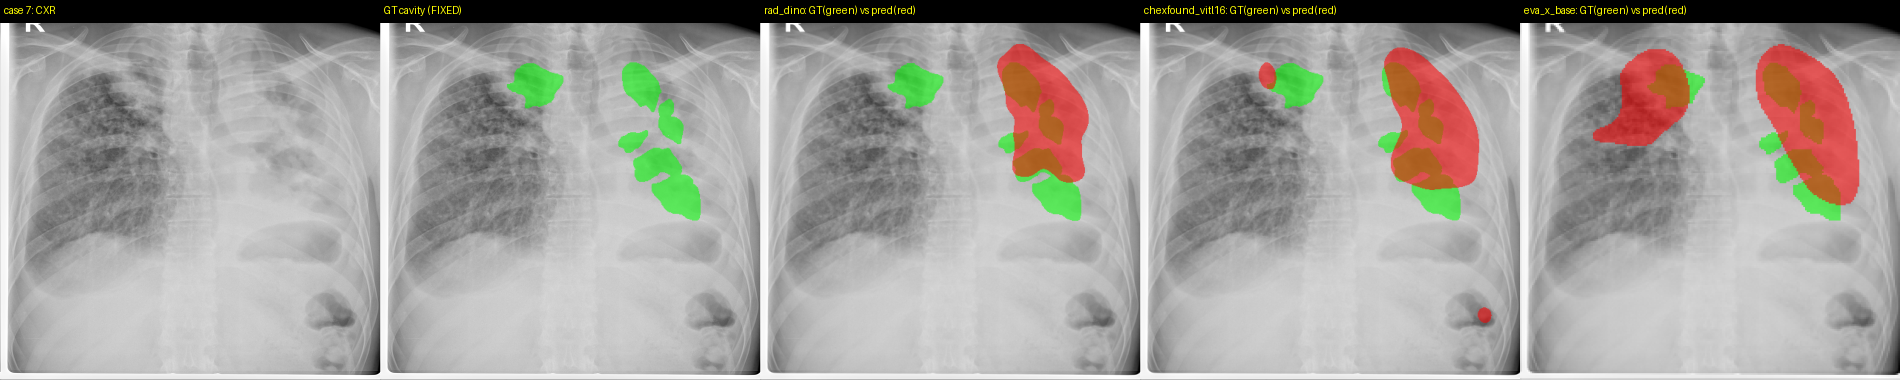
\includegraphics[width=\textwidth]{fig1_alignment_fix.png}
\caption{One test case, corrected ground truth (green) vs.\ each of the
three decoder ensemble members' predictions (red; orange = overlap). All
three members were already predicting a plausible, correctly-shaped lesion
region before the coordinate-frame fix -- the fix changes what the ground
truth is compared against, not the underlying predictions.}
\label{fig:overlay}
\end{figure}

Our foundation-decoder ensemble, however, showed an 8$\times$ dev/test Dice
cliff on first evaluation: $\approx$0.32--0.35 on the internal 89-image dev
slice, collapsing to $\approx$0.04 on the 111-case test set, for every one
of the three encoders individually and their ensemble. Three properties of
this collapse ruled out the two most likely causes in sequence:

\begin{enumerate}
\item \emph{Not a mis-tuned threshold.} Sweeping the binarization threshold
  directly against the already-computed test-set probability maps showed
  Dice remained flat at $\approx$0.04--0.05 across the \emph{entire} $[0.05,
  0.95]$ range -- a threshold problem would show recovery at some other
  operating point, and none was observed.
\item \emph{Not a corrupted or missing label.} Predicted-positive pixel
  counts were the same order of magnitude as ground-truth pixel counts for
  spot-checked cases (e.g.\ 10{,}538 predicted vs.\ 7{,}923 ground-truth
  pixels for one case) -- the model was confidently predicting a
  cavity-shaped region of plausible size, just not overlapping the
  annotation.
\item \emph{A coordinate-frame mismatch.} Sweeping array-level geometric
  transforms (transpose, four flips, four flip+transpose combinations)
  against the same fixed probability maps identified plain transpose as an
  outlier: $\approx$0.21--0.23 Dice, a $\sim$5$\times$ recovery, versus
  \emph{every} other candidate transform landing at $\le$0.06. This was
  confirmed both quantitatively (post-fix Dice reproduced through the
  corrected data-loading code, not just the diagnostic sweep) and visually
  (Fig.~\ref{fig:overlay} illustrative case: predictions and the
  \emph{corrected} ground truth agree closely once the transpose is
  applied).
\end{enumerate}

The root cause: ground-truth masks for the held-out test cases were sourced
from an nnU-Net-format conversion of the same annotations
(\texttt{nnUNet\_raw/.../labelsTr}), stored as fixed $512\times512$ arrays
regardless of each image's native resolution, with rows and columns swapped
relative to how the raw acquisition images are read by our own (SimpleITK)
image loader. Our internal dev split never touched this label store --
its masks were generated directly at native resolution alongside their
images and needed no transpose -- so the defect was invisible until the
test-only evaluation path was inspected directly. We fixed this by adding an
explicit \texttt{transpose} flag to every code path that reads
\texttt{labelsTr} (evaluation, ensembling, and a not-yet-run YOLOv8-seg
ancillary experiment that shared the same latent defect), applied only to
that label source.

\begin{table}[t]
\centering
\caption{Segmentation, held-out test set (n=111). ``Pre-fix'' / ``Post-fix''
refer to the ground-truth coordinate defect of Sect.~\ref{sec:pitfall}.}
\label{tab:seg}
\begin{tabular}{lc}
\toprule
Model & Test Dice \\
\midrule
nnU-Net baseline (2D, default plans)          & 0.306 \\
RAD-DINO decoder, pre-fix / post-fix          & 0.042 / 0.210 \\
CheXFound decoder, pre-fix / post-fix         & 0.044 / 0.206 \\
EVA-X-base decoder, pre-fix / post-fix        & 0.042 / 0.229 \\
+ dev-tuned threshold \& conn.-component filter & 0.213 / 0.203 / 0.213 \\
3-member ensemble, post-fix                   & 0.212 \\
\bottomrule
\end{tabular}
\end{table}

Post-fix single-encoder Dice ($\approx$0.21--0.23) remains below the internal
dev-slice number ($\approx$0.32--0.35) and below nnU-Net's baseline. We
attribute the residual gap to genuine train/test generalization on 444
training images rather than a further pipeline defect: (i) the same
label-source correction, applied identically to nnU-Net's own end-to-end
loop, produced \emph{no} change (Table~\ref{tab:seg}, row 1, already
self-consistent), and (ii) direct probability-map inspection across a
range of cases shows a mix of genuine model imprecision (partial-overlap
boundary error) and outright false-positive predictions in the
contralateral lung -- an error mode connected-component postprocessing is
designed to address. We swept binarization threshold jointly with a
minimum-component-size filter and an optional keep-top-$k$-components rule
on the dev slice only, then applied the dev-selected configuration to test:
the result was flat-to-slightly-worse relative to the untuned
threshold-0.5/no-filtering baseline for all three encoders (Table~\ref{tab:seg}),
indicating the residual gap is not simply solved by postprocessing the
existing probability maps, and is more likely a genuine small-data
generalization limit. The 3-member ensemble (0.212) also does not exceed
the strongest single member (EVA-X-base, 0.229) -- with only three members
and this much train/test generalization gap already present in each, they
are insufficiently diverse to help one another, unlike the free gains
typically reported for larger, more diverse ensembles in the literature. A
further dev-only sweep over per-member ensemble weights (rather than uniform
averaging) found a dev-dice-optimal configuration that dropped one member
entirely and reweighted the others (dev Dice 0.348 $\to$ 0.366), but this
improvement did not transfer to test (0.2121, statistically indistinguishable
from the uniform-weight ensemble's 0.2119) -- further evidence that the
89-image dev slice is too small to reliably guide decisions that generalize,
rather than a sign further tuning would help. Classifier-gating the
segmentation output (emitting an empty mask whenever the classifier predicts
cavity-negative) was also measured directly and found to slightly
\emph{reduce} Dice (e.g.\ EVA-X-base: 0.229 $\to$ 0.222), since the
classifier's $\approx$15\% error rate erases more genuine detections (false
negatives) than it removes false-positive noise (true negatives) -- we
nonetheless ship the gated configuration in the submission container for
output self-consistency (classifier and segmentation should not visibly
contradict each other) rather than the marginally higher raw-Dice ungated
alternative.

\subsection{Composite score}

Using the strongest single segmentation member (EVA-X-base), composite $=
0.7 \times 0.8468 + 0.3 \times 0.229 \approx 0.661$; using the 3-member
ensemble instead, $\approx 0.656$ -- within the noise band for $n=111$, but
we report both rather than only the more flattering number. This is
substantially more honest than the pre-fix pipeline would have reported
($\approx 0.7 \times 0.8468 + 0.3 \times 0.04 \approx 0.605$ either way), and
we regard the diagnostic process in
Sect.~\ref{sec:pitfall} as reusable practice: (a) compare dev and test
metrics computed via \emph{different} ground-truth sources for a
suspiciously large gap; (b) check whether a metric collapse is
threshold-invariant, which rules out calibration explanations; (c) compare
predicted vs. ground-truth \emph{pixel counts}, not just the resulting
score, to distinguish ``model predicts nothing'' from ``model predicts the
wrong place''; (d) when (c) indicates the latter, sweep coordinate
transforms directly against already-computed probability maps -- this
requires no retraining and isolates the defect to data loading rather than
modeling.

\section{Conclusion}

We present a classifier-gated foundation-model ensemble for TB cavity
classification and segmentation, and report an evaluation-pipeline defect
-- a coordinate-frame mismatch between an nnU-Net-derived label store and an
independently-loaded image pipeline -- that silently capped measured
segmentation performance at a small fraction of the model's true accuracy.
Beyond our own corrected numbers, we offer the diagnostic sequence in
Sect.~\ref{sec:pitfall} as a checklist for any project that mixes an
nnU-Net-format label store with a non-nnU-Net inference pipeline, a
combination we expect to be common as more work adapts foundation-model
encoders to nnU-Net-benchmarked segmentation tasks. Remaining open work:
connected-component postprocessing and a properly dev-tuned binarization
threshold against the \emph{corrected} labels (both in progress), and lung-ROI
cropping prior to decoding, which the wrong-lung false-positive pattern we
observed suggests could materially help.

\begin{thebibliography}{14}

\bibitem{who2023}
World Health Organization: Global Tuberculosis Report 2023. WHO, Geneva
(2023).

\bibitem{raddino}
P\'erez-Garc\'ia, F., et al.: RAD-DINO: Exploring Scalable Medical Image
Encoders Beyond Text Supervision. arXiv:2401.10815 (2024).

\bibitem{chexfound}
CheXFound: A Chest X-Ray Foundation Model with Global and Local
Representation Integration. (2024/2025).

\bibitem{evax}
EVA-X: A Foundation Model for General Chest X-ray Analysis with
Self-supervised Learning. (2024).

\bibitem{lora}
Hu, E.J., et al.: LoRA: Low-Rank Adaptation of Large Language Models. ICLR
(2022).

\bibitem{corn}
Shi, X., Cao, W., Raschka, S.: Deep Neural Networks for Rank-Consistent
Ordinal Regression Based on Conditional Probabilities. arXiv:2111.08851
(2021).

\bibitem{focaltversky}
Abraham, N., Khan, N.M.: A Novel Focal Tversky Loss Function with Improved
Attention U-Net for Lesion Segmentation. IEEE ISBI (2019).

\bibitem{nnunet}
Isensee, F., Jaeger, P.F., Kohl, S.A.A., Petersen, J., Maier-Hein, K.H.:
nnU-Net: a self-configuring method for deep learning-based biomedical image
segmentation. Nature Methods 18, 203--211 (2021).

\bibitem{densenet}
Huang, G., Liu, Z., van der Maaten, L., Weinberger, K.Q.: Densely Connected
Convolutional Networks. CVPR (2017).

\bibitem{effnetv2}
Tan, M., Le, Q.: EfficientNetV2: Smaller Models and Faster Training. ICML
(2021).

\bibitem{resnet}
He, K., Zhang, X., Ren, S., Sun, J.: Deep Residual Learning for Image
Recognition. CVPR (2016).

\bibitem{timm}
Wightman, R.: PyTorch Image Models. GitHub repository,
\url{https://github.com/rwightman/pytorch-image-models} (2019).

\end{thebibliography}
\end{document}